\myChapter{Distributed Evolutionary Algorithms}\label{chap:dEAs}
\minitoc\mtcskip
\vfill
\lettrine{T}{he} term Evolutionary Algorithm \cite{} is used to describe computer-based problem solving systems that use computational models whose design is based in evolution mechanisms. %CAMBIAR Y CITAR AL LIBRO DE EIBEN



\section{Types of Evolutionary Algorithm}

\begin{SaveVerbatim}{BasicEAtext}
BEGIN
 INITIALISE population with random candidate solutions;
 EVALUATE each candidate;
 REPEAT UNTIL (TERMINATION CONDITION is satisfied) DO
   1 SELECT parents;
   2 RECOMBINE pairs of parents;
   3 MUTATE the resulting offspring;
   4 EVALUATE new candidates;
   3 SELECT individuals for the next generation;
 OD
END
\end{SaveVerbatim}


\begin{SCfigure}[][!hb]
\begin{tabular}{|A|}
\hline
\BUseVerbatim{BasicEAtext}
\\
\hline
\end{tabular}
\caption{General scheme of an evolutionary algorithm in pseudo-code}
\label{tab:basicscheme}
\end{SCfigure}



\subsection{Genetic Algorithms}

\definicion{GAs}{Genetic Algorithms} are a type of optimization algorithms THAT %EIBEN
These kind of algorithms were proposed by \citep{holland1975adaptation}, and also studied by 

\subsection{Evolution Strategies}

\subsection{Genetic Programming}

\subsection{Evolutionary Programming}


\section{Parallel and Distributed Evolutionary Algorithms models}

\lettrine{T}{wo} main types of parallelization models for EAs are classified by \person{Alba and Tomassini} in \cite{alba2002parallelism}: \textsc{Global parallel EAs} and \textsc{Spatially structured EAs}.



\subsection{Global parallel evolutionary algorithms}%Farming model (centralized EAs) 
In this model, also called \textsc{Farming model} or \textsc{Centralized EAs}, the parallelism is applied at evaluation level, where a central node coordinate several slave nodes. The central node executes the EA in a sequential way, but distributes the individuals of the population to the slaves just for being evaluated. Figure \ref{fig:masterslave} depicts this situation.%An example can be seen in \cite{NUCLEAR}, where slave nodes evaluates fitness function for simullation of nuclear devices.

\begin{SCfigure}[20][htb]
\centering
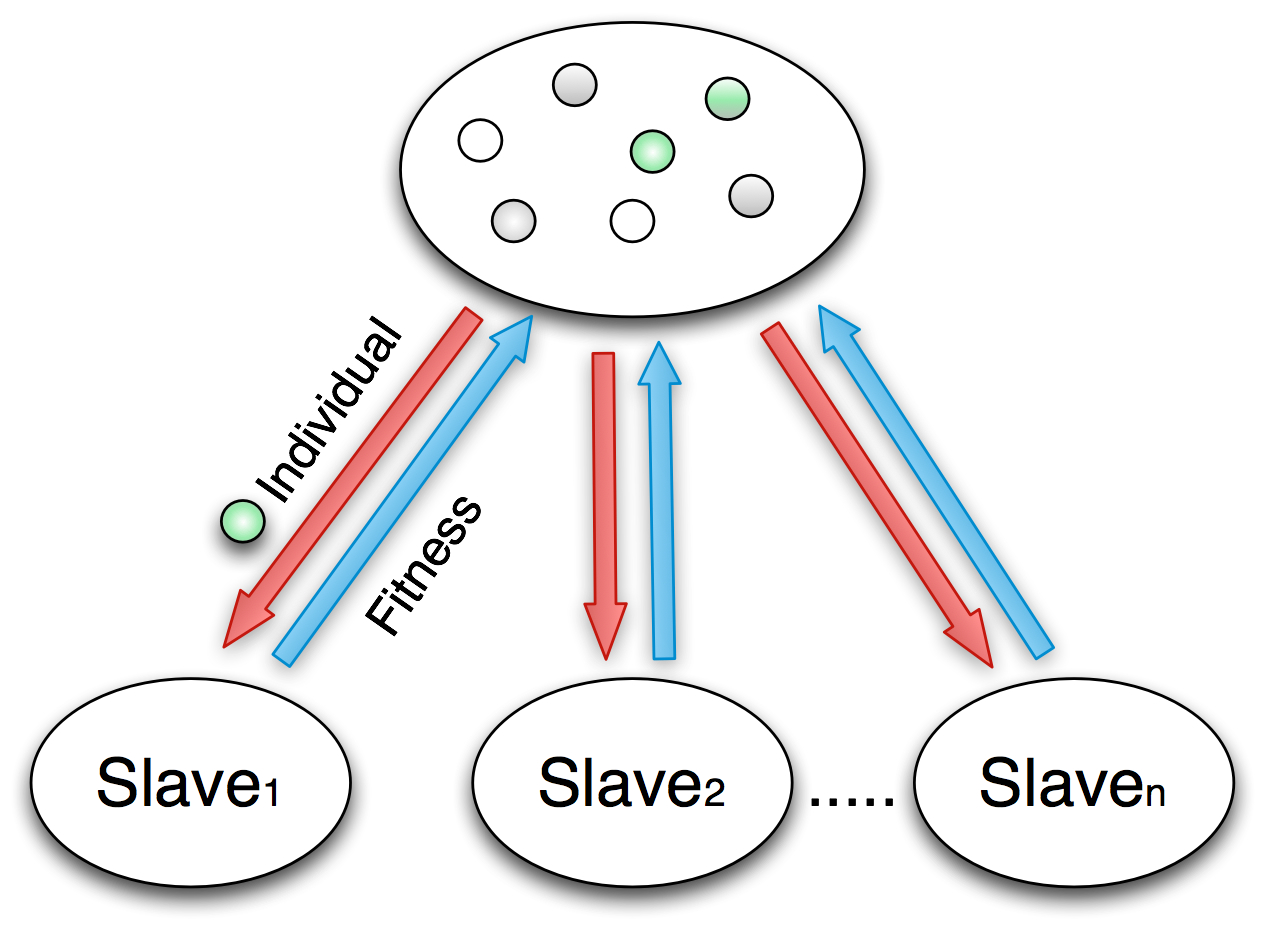
\includegraphics[width=26pc]{gfx/masterslave.jpg}
\caption{Master-slave model.}
\label{fig:masterslave}
\end{SCfigure}

\subsection{Spatially structured algorithms}%Island model (distributed EAs)
\subsubsection {Coarse-grained approach} One of the most usual approachs is the \textsc{Island model}, where a number of nodes executes simultaneously the EA, working with different sub-populations at the same time. Each certain number of generations is interchanged (migrated) between populations. Figure \ref{fig:ring} shows this model with a ring topology.

\begin{SCfigure}[20][htb]
\centering
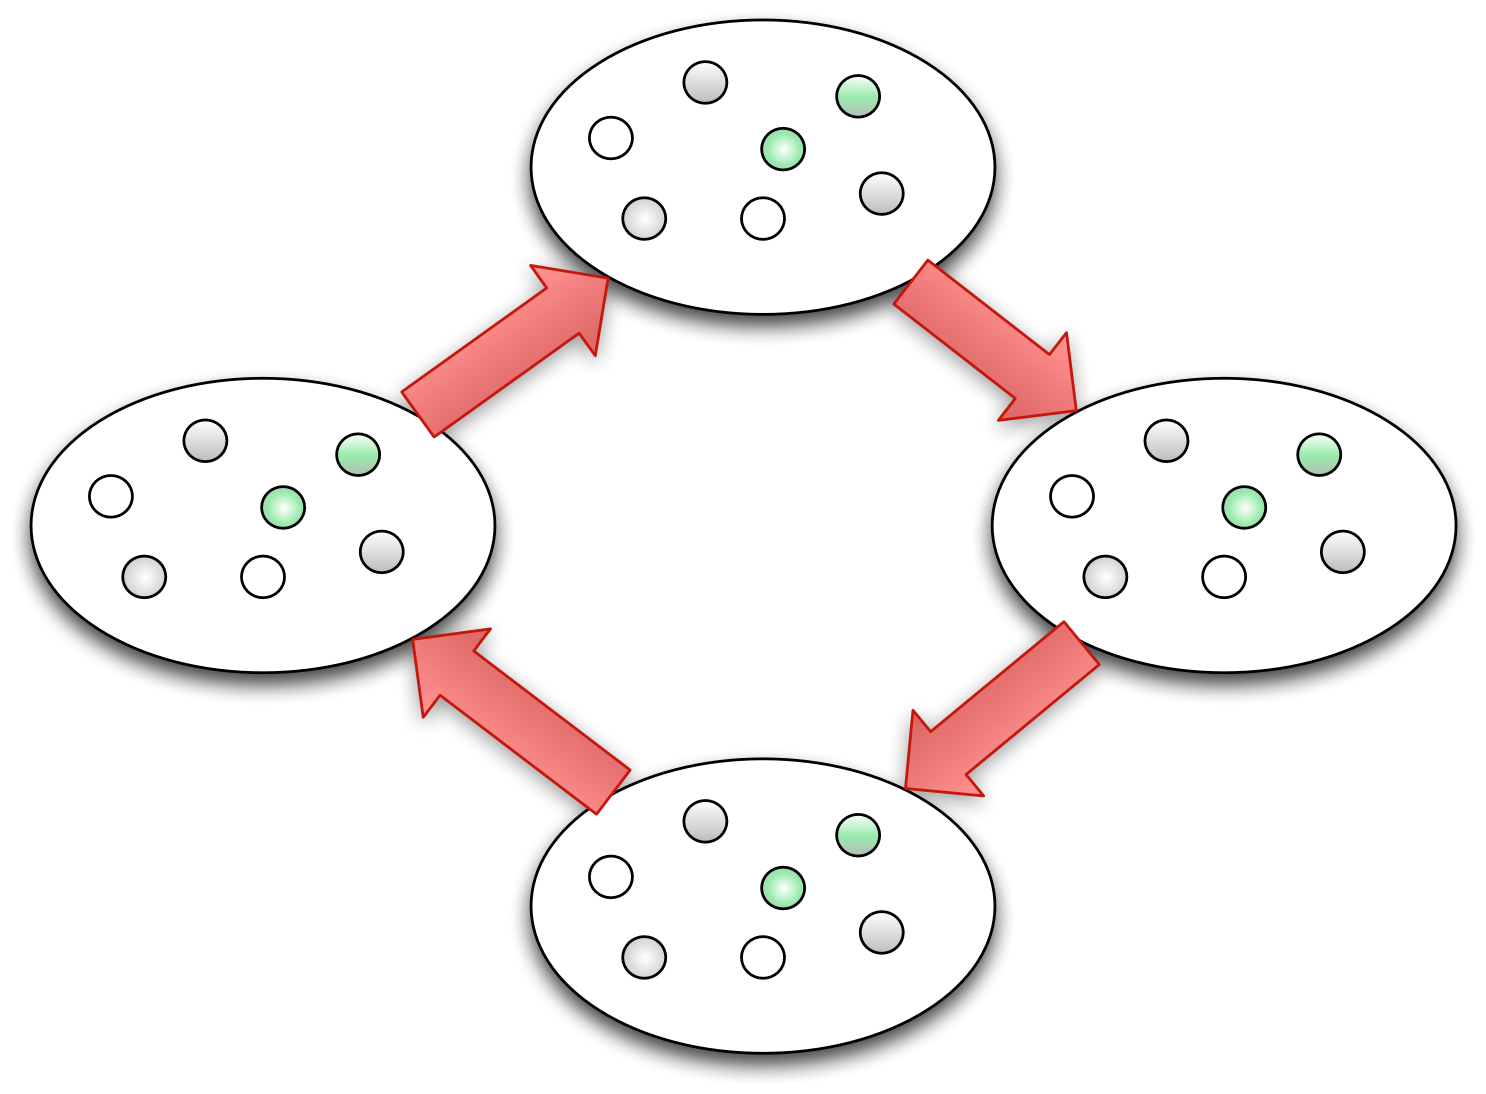
\includegraphics[width=26pc]{gfx/ring.jpg}
\caption{Island model scheme using a neighborhood ring topology.}
\label{fig:ring}
\end{SCfigure}

\subsubsection{Fine-grained approach}

In this approach, or Cellular EAs (CEAs) each node has one individual of the population, and selection and reproduction is limited with the individuals of the neighbourhood of the node \cite{CELLULAR}. Usually a bi-dimensional grid is used for topology, such as the one showed in the Figure \ref{fig:cellular}.

\begin{SCfigure}[20][htb]
\centering
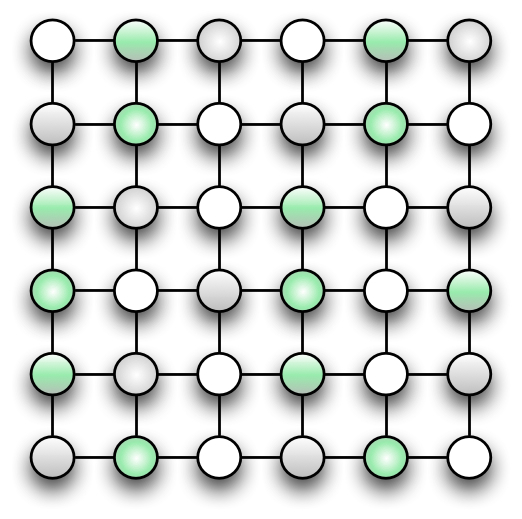
\includegraphics[width=5cm]{gfx/cellular.jpg}
\caption{Cellular Evolutionary Algorithm.}
\label{fig:cellular}
\end{SCfigure}

\subsection{Non-conventional approachs}
Appart from the previous approaches, new ones have been proposed, with the aim of new technologies, such as Cloud Computing, or the usage of heterogeneous hardware. For example, the \textsc{pool-based EAs} (p-EAs), where computational nodes exchange individuals using a shared pool. DECIR SQUE HAY EN EL POOL. This can lead to automatic load-balancing and synchronization, allowing the addition and removing of computers. Different technologies can be used, for example, in the work of \person{Meri \etal},  where the pool used is based in the Dropbox\texttrademark or SugarSync\texttrademark file storage services. Other authors propose the use of non-relational databases, such as the work of Merelo \etal \cite{merelo2010fluid}, using FluidDB. These databases allow...

%PREGUNTARLE A JJ SI EL POOL ES
%a) Una isla y los tipos acceden
%b) Una manera de intercambiar individuos

In \cite{merelo2012pool} the same authors improve the design, proposing an asynchronous, fault-tolerant, and scalable dEA, based on the object store CouchDB. The results show that adding clients could not scaly, but increase the fault tolerance. Also, their experimentation shows a good methodology for designing EAs in heterogeneous distributed systems, which have the impossibility of analytic performance prediction.

\definicion{P2P}{Peer-to-peer} systems are parallel infrastructures composed by a large number of resources, without any central server \cite{steinmetz2005peer}. The resources in this networks can appear or disappear dynamically. This platforms can be used to execute large instances of problems, taking advantage of the massive scalability that these systems offer. \definicion{EvAg}{Evolvable Agent}�\cite{laredo2010evag} creates a decentralised population, where every peer has a single individual, and new individuals are created combining the ones in their current neighbors. The population structure is maintained using the \textsc{newcast} protocol \cite{jelasity2003newscast}: each node has a cache of neighbours that can interchanged and combined. Figure \ref{fig:evag} shows this algorithm and population structure. Results show that this algorithm outperforms tuned GAs, using less links that a panmictic population. 

\begin{SCfigure}[20][htb]
\centering
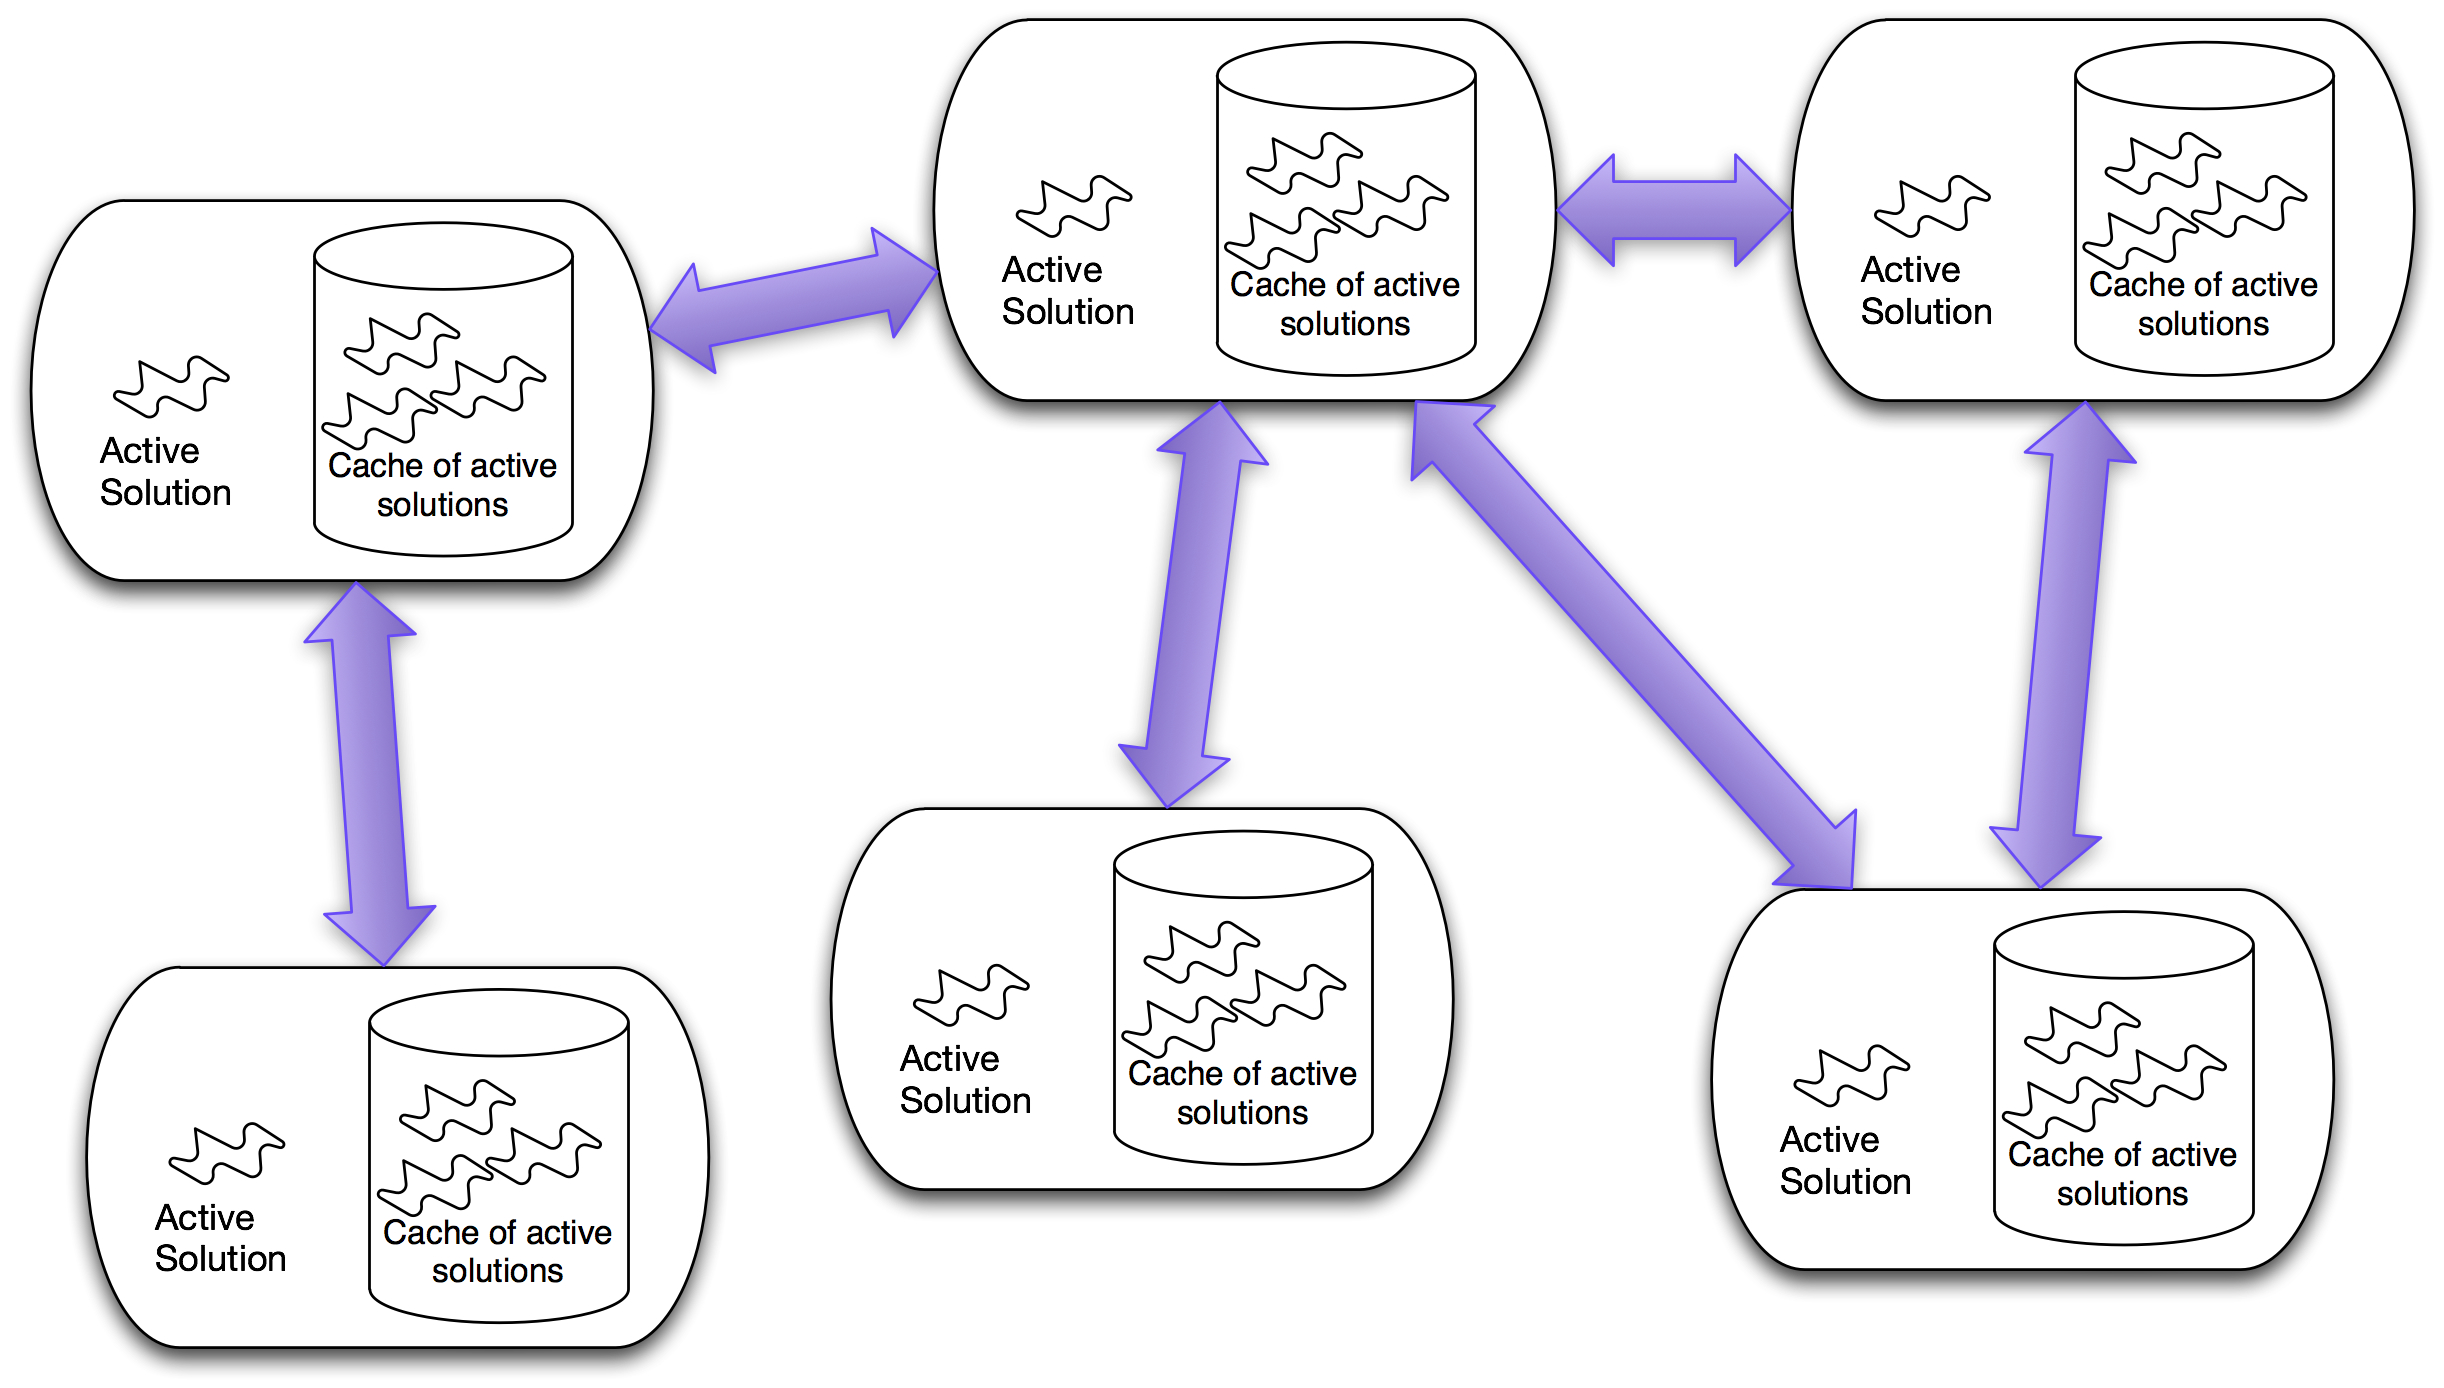
\includegraphics[width=26pc]{gfx/evag.jpg}
\caption{P2P Evolutionary Algorithm: EvAg.}
\label{fig:evag}
\end{SCfigure}



\section{Frameworks for Evolutionary Algorithms}
%%DECIR QUE HAY MUCHOS FRAMEWORKS ACTUALMENTE
In \cite{GENERICITY05}, \person{Gagn{\'e} and Parizeau} presented six criteria for qualify EA frameworks: generic representation, fitness, operator, model, parameters management and configurable output. In this work we show how SOA follows these lines of genericity, but can also extend them:
\begin{itemize}
\item Genericity in the service interfaces: service interfaces are established to create new implementations. Furthermore, these interfaces must be abstract enough to avoid their modification.
\item Programming language independence: for example, services implemented in Java can use services implemented in C++ and vice-versa.
\item Distribution transparency: it is not mandatory to use a specific library for the distribution, or modify the code to adapt the existing operators.
\item Flexibility: easy to add and remove elements to use the self-adaptation or other mechanisms.
\end{itemize}

Even as SOA is used extensively in software development, it is not widely accepted in the main EA software. 

\subsection{Object Oriented Frameworks}
Firstly, there exist
Object Oriented frameworks, such as Al\-go\-rithm::Evo\-lu\-tionary \citep{PERL},
\definicion{JCLEC}{Java Class Library for Evolutionary Computation} \citep{JCLEC} or jMetal \citep{JMETAL}. 
 Users implement specific interfaces of these frameworks (such as {\em
   individual} or {\em crossover}) and they group them in the source
 code. For example, creating an operator object that groups several
 operators. However, these frameworks are not compatible among them.
 For example, the operators created in JCLEC can not be used in jMetal
 (despite both are programmed in Java). Also, they can not control the
 services (operators) outside the source code.

\subsection{Parallel frameworks} 
Parallelism and distribution have been added to other frameworks, such as
MALLBA \citep{MALLBA}, \definicion{DREAM}{Distributed Resource Evolutionary Algorithm Machine} \citep{DREAM} or \definicion{ECJ}{Evolutionary Computation in Java} \citep{ECJ}, but
using external libraries (such as \definicion{MPI}{Message Passing Interface} or \definicion{DRM}{Distributed Resource Machine}), so the code that uses these
libraries is mixed with the algoritmh's code.


 Even being distributed, these frameworks can not communicate with each other. HeuristicLab \citep{HEURISTICLAB} is one of the few plug-in and service oriented frameworks. It uses web services for communication, but just to distribute the load, after consulting a central database of available jobs. Finally, the only service oriented optimization framework is GridUFO \citep{GRIDUFO}, but it only allows the modification of the objective function and the addition of whole algorithms, without combining existing services.  Table \ref{tab:frameworks} shows a summary of the previous frameworks.


\begin{SCtable}[][t]
\resizebox{11cm}{!}{
\begin{tabular}{llllll}
\hline
\rowcolor{colorCorporativoSuave}Name		&  Design 	 & Language 	& Distribution 	& License  		& Other	\\
\hline\hline
\rowcolor{colorCorporativoMasSuave}ECJ		& OO		& Java		& Sockets   	& Academic Free Lic. 	& Recently updated		\\
\rowcolor{colorCorporativoSuave}MALLBA		& OO		& C++		& MPI		& Freeware		& No new versions	\\
\rowcolor{colorCorporativoMasSuave}jMetal		& OO		& Java		& N/A		& GNU/LGPL 		&		\\
\rowcolor{colorCorporativoSuave}DREAM		& OO		& Java		& DRM		& GNU/GPL   		& No new versions		\\
\rowcolor{colorCorporativoMasSuave}ParadiseEO	& OO		& C++		& MPI		& CeCILL	   	&		\\
\rowcolor{colorCorporativoSuave}HeuristicLab	& OO/PO 	& .NET		& Web-Services	& GNU/GPL		& Recently updated			\\
\rowcolor{colorCorporativoMasSuave}METCO		& OO		& C++		& MPI		& N/A	   		&	\\
\rowcolor{colorCorporativoSuave}JCLEC		& OO		& Java		& N/A		& GNU/GL   		&	\\
\rowcolor{colorCorporativoMasSuave}Algorithm::Evol.& OO		& Perl		& N/A		& GNU/GPL  		& 	\\
\rowcolor{colorCorporativoSuave}GridUFO		&SO		& Java		& Web Services	& N/A  			& 	\\
\hline
%OSGiLiath	&OO/SO/PO 	& 2010			& Java		& Distributed OSGi	& GNU/GPL  	& Lifecycle management	\\
\end{tabular}
}
\caption{Comparison of EA frameworks. OO=Object-Oriented, SO=Service Oriented, PO=Plug-in Oriented}
\label{tab:frameworks}
\end{SCtable}

In brief, although these frameworks follows the six criteria for genericity proposed in \cite{GENERICITY05}, they present some shortcomings when it is needed to develop
or add new features: the user is forced to modify the source code
or stop the execution to add new functionalities (like load balancing,
dynamic control of operators, or an user interface). The authors should
improve their frameworks adding SOA technologies in order to facilitate the
communication and integration among them. As \person{Parejo \etal}  suggest in \cite{SURVEYMOFS}, a standardization of the presented (and other) frameworks should be carried out.


